\documentclass[handout]{beamer}
\usepackage{amsmath,amssymb,amsthm,array}
\usepackage{bm}
\usepackage{multirow}
\usepackage{multicol}
\usepackage{algorithm}
\usepackage{hyperref}
\usepackage{algorithmic}
\usepackage[normalem]{ulem}
\usepackage{fontspec}
\usepackage{numprint}
\usepackage{mathtools}
\DeclarePairedDelimiter{\ceil}{\lceil}{\rceil}
\setmainfont{CMU Serif}
\setsansfont{CMU Sans Serif}
\newfontfamily{\greekfont}{CMU Serif}
\newfontfamily{\greekfontsf}{CMU Sans Serif}

\usetheme{Rochester}
\usecolortheme{crane}
 
\setbeamertemplate{navigation symbols}{}

\title{Κρυπτοσυστήματα Διακριτού Λογαρίθμου}
\author{Παναγιώτης Γροντάς - Άρης Παγουρτζής}
\date{29/11/2016}
\defbeamertemplate*{footline}{shadow theme}
{%
  \leavevmode%
  \hbox{\begin{beamercolorbox}[wd=.5\paperwidth,ht=2.5ex,dp=1.125ex,leftskip=.3cm plus1fil,rightskip=.3cm]{author in head/foot}%
    \usebeamerfont{author in head/foot}\insertframenumber\,/\,\inserttotalframenumber\hfill  (\insertshortinstitute)
  \end{beamercolorbox}%
  \begin{beamercolorbox}[wd=.5\paperwidth,ht=2.5ex,dp=1.125ex,leftskip=.3cm,rightskip=.3cm plus1fil]{title in head/foot}%
    \usebeamerfont{title in head/foot}\insertshorttitle%
  \end{beamercolorbox}}%
  \vskip0pt%
}

\institute{ΕΜΠ - Κρυπτογραφία (2016-2017)}
 \hypersetup{
  pdfauthor={Panagiotis Grontas},
  pdftitle={Dlog},
  colorlinks=true,
  urlcolor=blue,
  linkcolor=white
}



\begin{document}

\setlength{\columnseprule}{0.4pt}

\newcommand{\xor}{ \oplus }
\newcommand{\MSG}{ \mathtt{M} }
\newcommand{\KEY}{ \mathtt{K} }
\newcommand{\CPH}{ \mathtt{C} }
\newcommand{\keygen}{\mathtt{KeyGen}}
\newcommand{\enc}{\mathtt{Encrypt}}
\newcommand{\dec}{\mathtt{Decrypt}}
\newcommand{\adv}{$\mathcal{A}$ }
\newcommand{\advb}{$\mathcal{B} \,$ }
\newcommand{\chal}{$\mathcal{C} \,$ }
\newcommand{\hash}{$\mathcal{H} \,$ }
\newcommand{\cs}{$\mathcal{CS} \,$ }
\newcommand{\zns}{  \mathbb{Z}^*_n }
\newcommand{\zn}[1]{  \mathbb{Z}^*_#1 }

\newcommand{\green}[1]{\textcolor{teal}{#1}}
\newcommand{\Green}[1]{\textcolor{Teal}{#1}}
\newcommand{\ForestGreen}[1]{\textcolor{ForestGreen}{#1}}
\newcommand{\blue}[1]{\textcolor{blue}{#1}}
\newcommand{\magenta}[1]{\textcolor{magenta}{#1}}
\newcommand{\cyan}[1]{\textcolor{cyan}{#1}}

\newcommand{\twopartdef}[4]
{ 
		\begin{cases}
			#1 , #2 \\
			#3 , #4
		\end{cases} 
}

\npthousandsep{ }
\begin{frame}
\titlepage
\end{frame}



\begin{frame}{Περιεχόμενα}
\begin{itemize}
\item Διακριτός Λογάριθμος: Προβλήματα και Αλγόριθμοι
\pause
\item Το κρυπτοσύστημα ElGamal
\pause 
\item Το κρυπτοσύστημα Cramer Shoup
\pause
\item Σχήματα Δέσμευσης με βάση το DLP
\pause
\item Ελλειπτικές Καμπύλες
\pause
\end{itemize}
\end{frame}


\section{DLP}
\begin{frame}[allowframebreaks]{Προβλήματα Διακριτού Λογαρίθμου}

\begin{block}{DLP - Το πρόβλημα του Διακριτού Λογαρίθμου}
Δίνεται μια κυκλική ομάδα $\mathbb{G}=<g>$ τάξης $q$ και ένα τυχαίο στοιχείο $y \in \mathbb{G}$

Να υπολογιστεί $x \in \mathbb{Z}_q$ ώστε $g^x = y$ \\
δηλ. το $log_g y \in \mathbb{Z}_q$
\end{block}

\begin{block}{CDHP - Το υπολογιστικό πρόβλημα Diffie Hellman}
Δίνεται μια κυκλική ομάδα $\mathbb{G}=<g>$, δύο στοιχεία $y_1=g^{x_1}, y_2 = g^{x_2}$

Να υπολογιστεί το $g^{x_1 \cdot x_2}$ 
\end{block}


\framebreak

\begin{block}{DDHP - Το πρόβλημα απόφασης Diffie Hellman}
Δίνεται μια κυκλική  ομάδα $\mathbb{G}=<g>$, δύο στοιχεία $y_1=g^{x_1}, y_2 = g^{x_2}$ και κάποιο  $y \in \mathbb{G}$ 

Να εξεταστεί αν  $y = g^{x_1 \cdot x_2}$ 
\end{block}
ή ισοδύναμα
\begin{block}{DDHP - Το πρόβλημα απόφασης Diffie Hellman}
Δίνεται μια κυκλική  ομάδα $\mathbb{G}=<g>$, δύο στοιχεία $y_1=g^{x_1}, y_2 = g^{x_2}$ και κάποιο  $y \in \mathbb{G}$ 

Μπορούμε να ξεχωρίσουμε τις τριάδες ($g^{x_1}, g^{x_2}, g^{x_1x_2}$) και  ($g^{x_1}, g^{x_2}, y$);
\end{block}
\end{frame}

\begin{frame}{Σχέσεις Προβλημάτων}
\begin{block}{$CDHP \leq DLP$}
Αν μπορούμε να λύσουμε το $DLP$, τότε μπορούμε να υπολογίζουμε τα $x_1, x_2$ από τα $y_1, y_2$ και στην συνέχεια το $g^{x_1 \cdot x_2}$
\end{block}

\pause
 
\begin{block}{$DDHP \leq CDHP$}
Αν μπορούμε να λύσουμε το $CDHP$, υπολογίζουμε το $g^{x_1 \cdot x_2}$ και ελέγχουμε ισότητα με το $y$
\end{block}
 
\pause 
Δηλαδή: $DDHP \leq CDHP \leq DLP$
\end{frame}
 
\begin{frame}{Επιλογή Ομάδας}
\begin{itemize}
    \item Καθορίζει τη δυσκολία του προβλήματος 
    \item Δύο επιλογές:
    \begin{itemize}
        \item $(\mathbb{Z}_p^*, \cdot)$ με $p$ πρώτο (σε υποομάδα)
        \item $(\mathcal{E}(\mathtt{F}_p),+)$
    \end{itemize}
    \item Διαφορετική παράμετρος ασφάλειας
    \item Κατά τα άλλα ισοδύναμες
\end{itemize}
\end{frame}



\begin{frame}{Αλγόριθμοι DLP}
\begin{block}{Brute Force}
Για ομάδα $\mathbb{G}=<g>$ τάξης $q$ $\lambda$ bits
\medskip

Δοκιμή όλων των $x \in \mathbb{Z}_q$ μέχρι να βρεθεί τέτοιο ώστε $g^x = y$
\medskip

Πολυπλοκότητα $O(2^\lambda)$
\end{block}
\end{frame}

%\begin{frame}{Σχέση με γεννήτορα}
%\begin{block}{Η δυσκολία του DLP είναι ανεξάρτητη από την επιλογή του γεννήτορα}
%Έστω $g_1, g_2$ γεννήτορες του $\mathbb{Z}_p^*$
%
%Για κάποιο $y \in \mathbb{Z}_p^*$: $y = g_1^x$ και $y=g_2^z$
%
%Δηλαδή: $g_1^x = g_2^z=(g_1^w)^z$
%
%Άρα: $x = wz \pmod{p-1} \Rightarrow z = xw^{-1} \pmod{p-1}$
%
%\end{block}
%Αν το DLP,μπορεί να επιλυθεί σε μία βάση - γεννήτορα, τότε μπορεί να υπολογιστεί σε οποιαδήποτε.
%\end{frame}

\begin{frame}{Αλγόριθμος Baby step - Giant Step (Shanks)}
Αλγόριθμος \green{Meet-In-The Middle}
\begin{itemize}
\item Ισχύει $x = ak-b, \, \,  k \in \mathbb{Z}, \, \forall x \in \mathbb{Z}$ 
\pause
\item $y=g^{ak} \cdot g^{-b} \Rightarrow \green{{y}{g^b}=g^{ak}}$
\pause
\item Θα υπολογίζουμε $yg^b$ και $g^{ak}$ μέχρι να συναντηθούν
\pause
\begin{itemize}
\item Ξεκινάμε στη 'μέση': $k = \ceil{\sqrt{q}}$\pause
\item \textbf{Giant steps - μέγεθος $k$}:Υπολογίζουμε ${g^{ak}}, a \in \{0 \cdots \ceil{\sqrt{q}}-1 \}$ και αποθηκεύουμε σε πίνακα \pause
\item \textbf{Baby steps - μέγεθος $1$}: Υπολογίζουμε $yg^b, b \in \{0 \cdots \ceil{\sqrt{q}}-1 \}$  μέχρι να βρούμε το αποτέλεσμα στον παραπάνω πίνακα \pause
\item $x = ak-b$
\end{itemize}
\end{itemize}
Πολυπλοκότητα χώρου και χρόνου: $O(2^\frac{\lambda}{2})$

Μείωση χώρου με αλγόριθμους Pollard ($\rho, \lambda$)
\end{frame}

\begin{frame}{Παράδειγμα Baby step - Giant Step}
\begin{block}{Θέλουμε το $2^x = 17 \pmod{29}$ στο $\mathbb{Z}_{29}^*=<2>$}
$\ceil{\sqrt{29}} = 6$
\pause
\begin{columns}
\column{0.5\textwidth}
\begin{itemize}
\item $2^{0 \cdot 6} = 1  \pmod{29}$
\pause
\item $2^{1 \cdot 6} = 6  \pmod{29}$
\pause
\item $2^{2 \cdot 6} = 7  \pmod{29}$
\pause
\item $2^{3 \cdot 6} = 13  \pmod{29}$
\pause
\item $2^{4 \cdot 6} = 20  \pmod{29}$
\pause
\item $2^{5 \cdot 6} = 4  \pmod{29}$
\end{itemize}
\pause
\column{0.5\textwidth}
\begin{itemize}
\item $17 \cdot 2^{0} = 17  \pmod{29}$
\pause
\item $17 \cdot 2^{1} = 5  \pmod{29}$
\pause
\item $17 \cdot 2^{2} = 10  \pmod{29}$
\pause
\item \green{$17 \cdot 2^{3} = 20  \pmod{29}$}
\end{itemize}
\end{columns}
\pause
\begin{center}
Άρα $x = 24-3 = 21$\\
Πράγματι: \green{$2^{21} = 17 \pmod{29}$}
\end{center}
\end{block}

\end{frame}

\begin{frame}{Αλγόριθμος Pohlig-Hellman - Ιδέα}

\begin{block}{Παρατήρηση}
Η δυσκολία του DLP σε μια ομάδα $\mathbb{G}$ εξαρτάται από τη δυσκολία του στις διάφορες υποομάδες της.
\end{block}
\pause
\begin{block}{Πώς}
Παραγοντοποίηση της τάξης

Για παράδειγμα στο $\mathbb{Z}_p^*$
\begin{center}
$p-1 = \prod_{i=1}^m p_i^{e_i}$ με $p_i$ πρώτο
\end{center}
\end{block}
\pause
\begin{block}{Smooth Number}
Μπορεί να παραγοντοποιηθεί σε μικρούς πρώτους
\end{block}
\end{frame}

\begin{frame}{Αλγόριθμος Pohlig-Hellman - Βήματα}
\begin{small}
Για κάθε μικρότερη ομάδα ($\bmod{p_i^{e_i}}$)
\begin{itemize}
\item Παρατηρούμε ότι $x_{p_i} = a_0+a_1p_i+\cdot+a_{e_i-1}p_i^{e_i-1} \pmod{p_i^{e_i}}$ με $a_j \in \{0,\cdots,p_{i}-1\}$ \pause
\item Πχ. αν παράγοντας του $p-1$ είναι το $4$: $x_2 = a_0 + a_1 *2 \pmod{4}$ \pause
\item Αποδεικνύεται (εύκολα) ότι: $y^\frac{p-1}{p_i} = g^{a_0\frac{p-1}{p_i}} \pmod{p}$ \pause
\item Υπολογισμός $a_0$ με δοκιμές ή με αλγόριθμο Shanks \pause
\item Δημιουργούμε ακολουθία $y_j$ με $y_0=y$ \pause
\item $y_{j} = y \cdot g^{-(a_0+a_1p_i+\cdot+a_{j-1}{p_i}^{j-1})} \pmod{p}$ \pause
\item Γενικεύοντας: $y_{j}^\frac{p-1}{p_i^{j+1}} = g^{a_j \frac{p-1}{p_i}}$ υπολογίζουμε το $a_j$ \pause
\item Υπολογισμός για κάθε $p_i$ : $ a_0, y_1, a_1, y_2, \cdots a_{e_i-1}$ \pause
\item Συνδυασμός λύσεων με CRT \pause
\end{itemize}
\end{small}
\end{frame}

\begin{frame}[allowframebreaks]{Παράδειγμα Pohlig-Hellman}
\begin{block}{Θέλουμε το $2^x = 17 \pmod{29}$ στο $\mathbb{Z}_{29}^*=<2>$}
$28=2^2 7$ \\
$x_2 = a_0 + 2a_1 \pmod{4}$ και $x_7 = a_0 \pmod{7}$ \\
\end{block}

\begin{block}{Υπολογισμός $a_0$ για το $x_2$}
$y^\frac{p-1}{2} = g^{a_0 \frac{p-1}{2}} \Rightarrow 17^{14} = 28 = 2^{14 a_0} \pmod{29}$ \\
Άρα $a_0=1$
\end{block}

\begin{block}{Υπολογισμός $y_1$ για το $x_2$}
$y_1 = y g^{-a_0} = 17 \cdot 2^{-1} = 17 * 15 = 23 \pmod{29} $
\end{block}

\framebreak

\begin{block}{Υπολογισμός $a_1$ για το $x_2$}
$y_1^\frac{p-1}{4} = g^{a_1 \frac{p-1}{2}} \Rightarrow 23^7 = 1 = 2^{14 a_1} \pmod{29}$\\
Άρα $a_1=0$ \\
\end{block}
Άρα \green{$x_2 = 1 \pmod{4}$}
 
\begin{block}{Υπολογισμός $a_0$ για το $x_7$}
$y^\frac{p-1}{7} = g^{a_0 \frac{p-1}{7}} \Rightarrow 17^4 = 1 = 2^{4 a_0} \pmod{29}$ \\
Άρα $a_0=0$
\end{block}

Άρα \green{$x_7 = 0 \pmod{7}$}
\\
Από CRT: $x = 21$

Πιο αναλυτικό  \href{http://www-math.ucdenver.edu/~wcherowi/courses/m5410/phexam.html}{παράδειγμα}
\end{frame}

\begin{frame}[allowframebreaks]{Δυσκολία DDHP}
\begin{small}
\begin{block}{Θεώρημα}
To DDHP δεν είναι δύσκολο στην $\mathbb{Z}_p^*$
\end{block}
\pause
Μπορεί να κατασκευαστεί αποδοτικός αλγόριθμος διαχωρισμού τριάδας DH $g^a,g^b,g^{ab}$ από μια τυχαία τριάδα $g^a,g^b,g^c$.\\
\pause
\magenta{Πώς:} Χρησιμοποιώντας το \green{σύμβολο Legendre.}
\pause
\begin{block}{To σύμβολο Legendre διαρρέει το DLP parity}
Από τον ορισμό: 
$(\frac{g^{x}}{p}) = (g^{x})^{\frac{p-1}{2}}$ \\
Όμως:
$g^{p-1} = 1 \pmod{p}$ \\
Άρα: 
$g^\frac{p-1}{2} = -1 \pmod{p}$ \\
Δηλαδή:
$(\frac{g^{x}}{p}) = (-1)^x$ \\
Αν $x$ μονός  τότε $(\frac{g^{x}}{p}) = -1$ ($g^x \not\in QR$)\\
Αν $x$ ζυγός  τότε $(\frac{g^{x}}{p}) = 1$  ($g^x \in QR$)
\end{block}
\pause
Για τυχαία τριάδα $Prob[(\frac{g^{c}}{p}) = 1] = \frac{1}{2}$ ανεξάρτητο από τα $(\frac{g^{a}}{p}),(\frac{g^{b}}{p})$\\
\pause
Για τριάδα DH: $Prob[(\frac{g^{ab}}{p}) = 1] = \frac{3}{4}$
\pause
\begin{block}{Ο αλγόριθμος}
Υπολόγισε $\frac{g^{c}}{p},\frac{g^{b}}{p},\frac{g^{c}}{p}$ \\
Αν $\frac{g^{c}}{p} = 1$ και $(\frac{g^{a}}{p} =1$  ή $\frac{g^{b}}{p} = 1)$ τότε \\
 $\>$$\>$$\>$  Επιστροφή "Diffie Hellman" \\
Αλλιώς \\
  $\>$$\>$$\>$ Επιστροφή "Τυχαία" \\
\end{block}
Πλεονέκτημα: $\frac{3}{8}$ (γιατί;) \\
\end{small}
\alert{ΜΗ ΑΜΕΛΗΤΕΟ}\\

\end{frame}

\begin{frame}{Επιλογή του $\mathbb{G}$}
\begin{small}
\begin{block}{Συνέπειες}
Δουλεύουμε σε μεγάλη υποομάδα του $\mathbb{Z}_p^*$ με τάξη πρώτο $q$
\end{block}
\pause
\begin{block}{Για παράδειγμα:}
Επιλογή safe prime: $p = 2q+1$ με $q$ πρώτο 

Δουλεύουμε στην υποομάδα τετραγωνικών υπολοίπων τάξης $q$

Επιλογή schnorr primes $p = k \cdot q+1$ με $q$ πρώτο

\alert{Παρ' όλα αυτά}: Yποεκθετικοί αλγόριθμοι (index calculus)
\end{block}
\pause
\begin{block}{Μεγέθη}
\begin{tabular}{ccc}
Symmetric Security & $|p|$ & $|q|$ \\
80 bits &  1024 & 160 \\
112 bits & 2048 & 224 \\
128 bits &  3072 & 256 \\
\end{tabular}
\end{block}
\pause
Εναλλακτικά: Ελλειπτικές καμπύλες
\end{small}
\end{frame} 

\section{Το κρυπτοσύστημα ElGamal}
\begin{frame}{Ορισμός ElGamal}
 
\textbf{Δημιουργία Κλειδιών:}
$KeyGen(1^{\lambda}) = (y=g^x,x)$
\begin{itemize}
\item Επιλογή δύο μεγάλων πρώτων $p,q$ ώστε $q \mid (p-1)$  
\item Δουλεύουμε στην υποομάδα τάξης q του $\mathbb{Z}_p^*$ $\mathtt{G}$ με γεννήτορα $g$
\item Επιλογή τυχαίου $x \in \mathbb{Z}_q$
\item Υπολογισμός $y = g^x \bmod{p}$
\item Επιστροφή $(y,x)$
\end{itemize}
\pause
 
\textbf{Κρυπτογράφηση} 
\begin{itemize}
\item Επιλογή τυχαίου $r \in \mathbb{Z}_q$
\item $\enc(y,r,m) = (g^r \bmod p, m \cdot y^r \bmod p)$
\end{itemize}
\pause

\textbf{Αποκρυπτογράφηση}
\begin{itemize}
\item $\dec(x, (a,b)) = \frac{b}{a^x}$
\end{itemize} 
\pause
 
\begin{block}{\magenta{Ορθότητα}}
$\dec(x, \enc(y,r,m))= \frac{m y^r}{(g^r)^x} = m$
\end{block}

\end{frame}

\begin{frame}{Πρακτικά Θέματα}

\green{Πιθανοτική Κρυπτογράφηση:} Ένα μήνυμα έχει πολλά πιθανά κρυπτοκείμενα \\
\pause
\alert{Message expansion} Κρυπτοκείμενο διπλάσιο του μηνύματος \\
\pause
\begin{block}{Επιτάχυνση Κρυπτογράφησης}
Κόστος: 2 υψώσεις σε δύναμη - 1 πολλαπλασιασμός\\
Ύψωση σε δύναμη:Δεν εξαρτάται από το μήνυμα (precomputation)
\end{block}

\end{frame}

\begin{frame}{Ασφάλεια Κρυπτογράφησης}
\begin{block}{ElGamal \equiv CDHP}
Αντιστοιχία δημοσίων στοιχείων
$g^{x_1} \equiv g^r$ \\
$g^{x_2} \equiv y=g^x$ \\
Υπολογισμός $g^{x_1x_2}$ $\rightarrow$ αποκρυπτογράφηση \\

Αν δεν μπορώ να αποκρυπτογραφήσω (χωρίς το κλειδί)\\ $\rightarrow$ δεν μπορώ να λύσω το $CDHP$
\end{block}
\end{frame}

\begin{frame}{Επανάληψη τυχαιότητας $\rightarrow$ Επίθεση KPA}
KPA: Γνωρίζουμε  ζεύγη μηνυμάτων - κρυπτοκειμένου 
\pause
\begin{block}{Επίθεση}
$(c_r,c_1) = \enc(y,r,m_1) = (g^r \bmod p, m_1 \cdot y^r \bmod p)$
$(c_r,c_2) = \enc(y,r,m_2) = (g^r \bmod p, m_2 \cdot y^r \bmod p)$
\end{block}
\pause
Αν γνωρίζω το $(m_1,c_1)$:
$c_1 = m_1 \cdot y^r \bmod p \Rightarrow y^r = c_1 \cdot m_1^{-1}$\\
\medskip
\pause
Μπορώ να υπολογίσω το $m_2$ ως:
$m_2 = \frac{c_2}{y^r} = \frac{c_2}{c_1 \cdot m_1^{-1}}$
\end{frame}

\begin{frame}[allowframebreaks]{Ασφάλεια σε επιθέσεις CPA}
\begin{block}{Θεώρημα}
Αν το DDHP είναι δύσκολο, τότε το κρυπτοσύστημα El Gamal διαθέτει ασφάλεια IND-CPA.
\end{block}

Απόδειξη:

Έστω ότι το ElGamal δεν διαθέτει ασφάλεια IND-CPA. 

Άρα $\exists$ \adv, ο οποίος μπορεί να νικήσει στο παιχνίδι CPA με μη αμελητέα πιθανότητα. 

Κατασκευή \advb:
\begin{itemize}
\item Είσοδος: τριάδα στοιχείων
\item Εσωτερικά: Προσομοίωση του \chal στο παιχνίδι CPA και χρήση \adv 
\item Αποτέλεσμα: Ξεχωρίζει DH τριάδα από τυχαία 
\end{itemize}
 


\begin{itemize}
\item Είσοδος: $g^\alpha,g^\beta, g^c$
\item Στο CPA-GAME δημόσιο κλειδί $y =  g^\alpha$ 
\item Ο \advb απαντά στις κρυπτογραφήσεις του \adv
\item Όταν ο \adv προκαλέσει με δύο μηνύματα 
\begin{itemize}
\item o \chal διαλέγει τυχαίο $bit \in \{0, 1\}$,
\item κρυπτογραφεί το $M_b$ με τυχαιότητα το $g^\beta$ και πολλαπλασιάζει με $g^{c}$
\item Τελικά στέλνει το:  $( g^\beta  , M_b \cdot g^{c}  )$
\end{itemize}
\item O \adv επιστρέφει την τιμή του ${bit}^*$
\item Ο \advb εξάγει το ${bit}^*$
\end{itemize}



\begin{block}{Ανάλυση}
\begin{itemize}

\item Για τριάδα DH: $g^c = (g^\alpha)^\beta = y^\beta $ 
\item ο \adv θα λάβει ένα έγκυρο κρυπτοκείμενο ElGamal.
\item H πιθανότητα να μαντέψει σωστά είναι τουλάχιστον: ${1}/{2} + \text{non-negl}(\lambda)$.

\item Για τυχαία τριάδα: ο \adv θα πρέπει να μαντέψει τυχαία
\item Πιθανότητα επιτυχίας: $\frac{1}{2}$.

\item Τελική πιθανότητα επιτυχίας για \advb τουλάχιστον $\text{non-negl}(\lambda)$
\item Μπορεί να ξεχωρίσει μία DH τριάδα από μία τυχαία με μη αμελητέα πιθανότητα.

\end{itemize}
\end{block}

\begin{center}
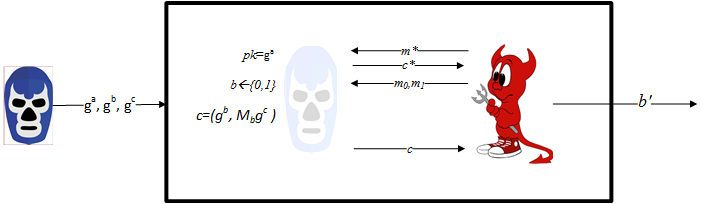
\includegraphics[height=7.15cm, width=11.5cm]{egcpa.png}
\end{center}

\end{frame}

\begin{frame}[allowframebreaks]{Ομομορφικές Ιδιότητες}

\begin{block}{Πολλαπλασιαστικός Ομομορφισμός}
\begin{align*}
\enc(y,r_1,m_1) \cdot \enc(y,r_2,m_2) = \\
(g^r_1, m_1 y^{r_1}) \cdot (g^r_2, m_2 y^{r_2}) =\\
(g^{r_1+r_2}, (m_1 \cdot m_2) \cdot y^{r_1+r_2}) = \\
\enc(y, r_1+r_2,m_1  m_2)
\end{align*}
\end{block}

\framebreak

\begin{block}{Reencryption}
\begin{align*}
\enc(y,r_1,m) \cdot \enc(y,r_2,1) = \\
(g^{r_1}, my^{r_1}) \cdot (g^{r_2},  y^{r_1}) =\\
(g^{r_1+r_2}, my^{r_1+r_2}) =
\enc(y,r_1+r_2,m) 
\end{align*}
\end{block}
\green{Αλλαγή της τυχαιότητας - Αλλαγή της μορφής του μηνύματος} \\
\alert{...χωρίς γνώση του ιδιωτικού κλειδιού} \\
\alert{Malleability}

\framebreak

\begin{block}{Προσθετικός Ομομορφισμός - Εκθετικό ElGamal}
Κρυπτογράφηση του $g^m$ 

$\enc'(y,r,m) = (g^r, g^m y^r)$

\begin{align*}
\enc'(y,r_1,m_1) \cdot \enc'(y,r_1,m_1) = \\
(g^r_1, g^{m_1} y^{r_1}) \cdot  (g^r_2, g^{m_2} y^{r_2}) =\\
(g^{r_1+r_2} , g^{m_1 + m_2} \cdot y^{r_1+r_2}) = \\
\enc(y,r_1+r_2,(m_1 + m_2))
\end{align*}

Αποκρυπτογράφηση: Λαμβάνουμε το $g^m$

\alert{Επίλυση 'εύκολου' διακριτού λογαρίθμου}.

\end{block}

\end{frame}

\begin{frame}{Ασφάλεια σε επιθέσεις CCA}
 
\begin{block}{To παραδοσιακό ElGamal δεν διαθέτει CCA-security}
Έστω ότι ο \adv  μπορεί να αποκρυπτογραφήσει μηνύματα επιλογής του, εκτός του $c$.
\begin{itemize}
\item Στόχος: Αποκρυπτογράφηση του $c = (G,M) = (g^r, m_b y^r)$
\pause
\item Κατασκευή $c' = (G',M') = (G \cdot g^{r'}, M \cdot a y^{r'}) = (g^{r+r'}, a \cdot m_b \cdot y^{r+r'}) $, όπου $a$ επιλέγεται από τον  \adv 
\pause
\item H αποκρυπτογράφηση του $M'$ ($\frac{M'}{G'^x}$) δίνει το $am_b$ και κατά συνέπεια το $m_b$
\pause
\item Αν $m_b = m_0$ επιστρέφει $b^*=0$ αλλιώς επιστρέφει $b^*=1$
\end{itemize}
\end{block}

\end{frame}

\section{Cramer-Shoup cryptosystem}
\begin{frame}[allowframebreaks]{ElGamal CCA2: Cramer-Shoup cryptosystem}
\begin{itemize}
\item Ronald Cramer, Victor Shoup, Crypto 1998
\item Επέκταση του ElGamal
\item Χρηση συνάρτησης σύνοψης \hash με collision resistance  (δεν είναι απαραίτητη)
\item Αν ισχυει η υπόθεση DDH, τότε παρέχει IND-CCA2
\end{itemize}

\begin{block}{Δημιουργία Κλειδιών}
\begin{itemize}
\item Επιλογή πρώτων $p,q$ με $p=2q+1$
\item $G$ ειναι η υποομάδα ταξης $q$ στο $\zn{p}$
\item Επιλογή random generators $g_1, g_2$

\item Επιλογή τυχαίων στοιχείων $x_1,x_2,y_1,y_2,z \in \mathbb{Z}_{q}$
\item Υπολογισμός
\begin{itemize} 
\item $c=g_1^{x_1}g_2^{x_2}$
\item $d=g_1^{y_1}g_2^{y_2}$
\item $h=g_1^{z}$
\end{itemize}
\item Δημόσιο Κλειδί: $(c,d,h)$
\item Μυστικό Κλειδί: $(x_1,x_2,y_1,y_2,z)$
\end{itemize}
\end{block}

\framebreak

\begin{block}{Κρυπτογράφηση}
\begin{itemize}
\item Κωδικοποίηση μηνύματος $m$ στο $G$
\item Επιλογή τυχαίου $r \in \mathbb{Z}_{q}$
\item Υπολογισμός
\begin{itemize} 
\item $u_1 = g_1^r,u_2 = g_2^r$
\item $e = m h^r$
\item $\alpha = $ \hash$(u_1||u_2||e)$
\item $v = c^r d^{r\alpha}$ 
\end{itemize}
\item Κρυπτογράφημα: $(u_1,u_2,e,v)$
\end{itemize}
\end{block}

\framebreak
\begin{block}{Αποκρυπτογράφηση}
\begin{itemize}
\item Υπολογισμός $\alpha = $ \hash$(u_1||u_2||e)$
\item Έλεγχος αν $u_1^{x_1}u_2^{x_2}(u_1^{y_1}u_2^{y_2})^\alpha=v$. Σε περίπτωση αποτυχίας έξοδος χωρίς αποκρυπτογράφηση
\item Σε περιπτωση επιτυχίας υπολογισμός $m = \frac{e}{u_1^z}$
\end{itemize}
\end{block}
\framebreak
\begin{block}{Ορθότητα}
$\frac{e}{u_1^z} = \frac{mh^r}{u_1^z} = m \cdot \frac{g_1^{zr}}{g_1^{rz}} = m$
\begin{itemize}
\item $h,z$ αντιστοιχούν σε δημόσιο - ιδιωτικό κλειδί  ElGamal
\item $u_1, e$ αντιστοιχούν στο κρυπτογράφημα του ElGamal
\end{itemize}
\end{block}

\begin{block}{Παρατηρήσεις}
\begin{itemize}
\item $u_2,v$ λειτουργούν ως έλεγχος ακεραιότητας, ώστε να  μπορεί να αποφευχθεί το malleability 
\item Διπλάσια πολυπλοκότητα από ElGamal τόσο σε μέγεθος κρυπτοκειμένου, όσο και σε υπολογιστικές απαιτήσεις
\end{itemize}
\end{block}
\end{frame}

\section{DLP-based Commitment Schemes}
\begin{frame}{DLP-based Commitment Schemes}
\begin{block}{Επανάληψη}
\begin{itemize}
\item Coin Flipping over the telephone
\pause
\item Λύση:  Commitment Schemes
\pause
\begin{itemize}
\item \textbf{Hiding} - Προστατεύει αποστολέα -  καθώς δεν μπορεί να διαρρεύσει η τιμή του
\pause
\item \textbf{Binding} - Προστατεύει παραλήπτη -  καθώς ο αποστολέας δεν μπορεί να αλλάξει την τιμή του εκ των υστέρων
\pause
\end{itemize}
\item Χρήση randomisation για προστασία από brute-force επιθέσεις
\end{itemize}
\end{block}
\end{frame}

\begin{frame}{Pedersen commitment}
\begin{itemize}
\item  Επιλογή ομάδας με δύσκολο DLP από TTP
\begin{itemize}
\item Επιλογή πρώτου $q$ ώστε $p=2q+1$ πρώτος
\item $\mathbb{G}=<g>$ υπομάδα τάξης $q$ του $\mathbb{Z}_p^*$
\item Επιλογή $x \in \mathbb{Z}_q$ και $h=g^x$
\item Δημοσιοποίηση $g,\mathbb{G},p,q,h$
\end{itemize}
\pause
\item Δέσμευση: $c=commit(m,r) = g^m \cdot h^r \bmod{p}$
\pause
\item Αποκάλυψη: Αποστολή $m,r$
\pause
\item Επαλήθευση: $c =_? g^m \cdot h^r$
\end{itemize}
\end{frame}

\begin{frame}[allowframebreaks]{Ιδιότητες}
\begin{block}{Information Theoretically Hiding}
$c = g^m \cdot h^r \bmod{p}=g^{m+xr} \bmod{p}$

Ακόμα και ένας παντοδύναμος αντίπαλος να μπορεί να λύσει το DLP θα έχει μία εξίσωση της μορφής

$d = m+xr \pmod{q}$ 

(2 άγνωστοι $m,r$ - 1 εξίσωση)
\end{block}

\framebreak

\begin{block}{Computationally Binding αν το DLP είναι δύσκολο}
Έστω $c=commit(m,r)=commit(m',r')$ με $m \neq m'$

\begin{align*}
g^m \cdot h^r = g^{m'} \cdot h^{r'} \Rightarrow \\
g^{m+xr} = g^{m' + xr'} \Rightarrow \\
m+xr=m'+xr' \pmod{q} \Rightarrow \\
x = \frac{m'-m}{r-r'}
\end{align*}

\alert{ΑΤΟΠΟ}
\end{block}
\end{frame}



\begin{frame}{Ελλειπτικές καμπύλες}
\begin{block}{Γενικά}
\begin{itemize}
\item Πλούσιο σε ιστορία μαθηματικό αντικείμενο (200 έτη) \pause
\item Κρυπτογραφία: 80s \pause
\item Βασίζονται στο πρόβλημα DLP \pause
\begin{itemize}
\item Αντικατάσταση του $\mathbb{Z}_{p}$ με σημεία τους \pause
\item Μόνο γενικευμένοι αλγόριθμοι DLP $O(2^\frac{\lambda}{2})$ - όχι υποεκθετικοί \pause
\item Ίδια επίπεδα ασφάλειας με μικρότερη παράμετρο ασφάλειας και καλύτερη απόδοση\\
\begin{tabular}{cc}
RSA & EC \\
1024 & 160 \\
2048 & 224 \\
3072 & 256 \\
\end{tabular}
\end{itemize}
\end{itemize}
\end{block}
\end{frame}

\begin{frame}{Γενική μορφή}
Έστω $\mathbb F$ ένα σώμα.
\pause
\begin{block}{Ορισμός $\mathcal{E}(\mathbb{F})$}
Mια ελλειπτική καμπύλη $\mathcal{E}$ πάνω από το $\mathbb F$ είναι το σύνολο των σημείων  $(x,y) \in \mathbb F$, που ικανοποιούν την εξίσωση Weierstrass 
\begin{align*}
y^2+a_1xy+a_3y=x^3+a_2x^2+a_4x+a_6 \\  a_1, a_2, a_3, a_4, a_5, a_6 \in \mathbb{F}
\end{align*}  
 και  ένα στοιχείο $\mathcal O$, - \emph{σημείο στο άπειρο}
\end{block}
\pause
\begin{block}{Πρακτικά} 
$
y^2=x^3+ax+b ,\ \ a, b \in \mathbb F\  
$

\end{block}
\end{frame}

\begin{frame}[allowframebreaks]{Ελλειπτικές καμπύλες στο $\mathbb R$}
\begin{figure}
\begin{tiny}
\begin{tabular}{cccc}
		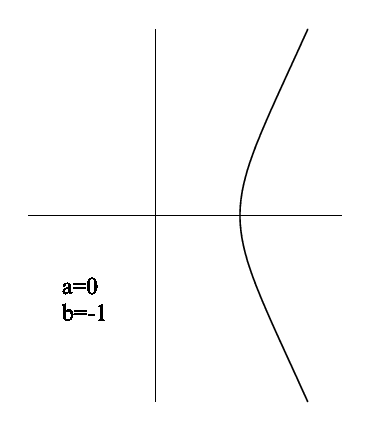
\includegraphics[scale=0.25]{qaz1.png} & $y^2 = x^3 - 1 $   &  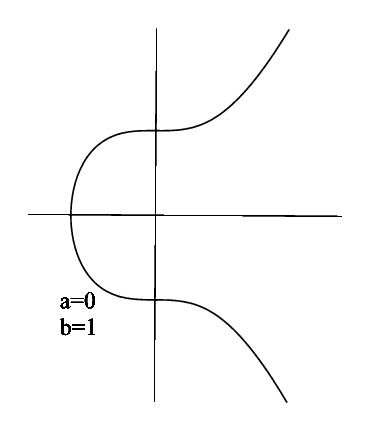
\includegraphics[scale=0.25]{qaz2.png} &  $y^2 = x^3 + 1 $ \\       
        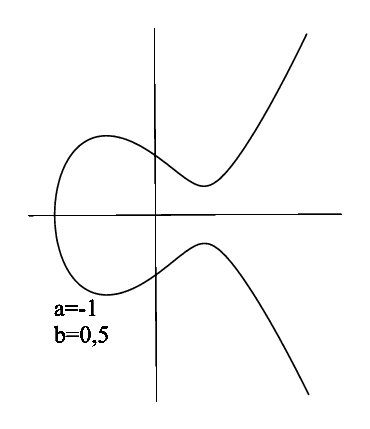
\includegraphics[scale=0.25]{qaz3.png} & $y^2 = x^3 - x +\frac{1}{2} $ &  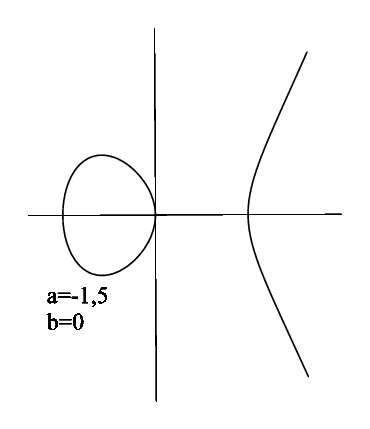
\includegraphics[scale=0.25]{qaz4.png}  &  $y^2 = x^3 - \frac{3}{2}x $
\end{tabular}
\end{tiny}
\end{figure}

\framebreak

Παρατηρήσεις:
\begin{itemize}
\item Συμμετρία ως προς άξονα $x$
\item Συμπίεση σημείου $(x,0)$ ή $(x,1)$ για πάνω ή κάτω από τον άξονα των $x$
\end{itemize}

\alert{Προς αποφυγή} Singular καμπύλες: Πολλαπλές ρίζες, σημεία τομής

\begin{figure}

\includegraphics[scale=0.3]{singular.png}
\end{figure}

Πρέπει $4a^3+27b^2 \neq 0$
\end{frame}

\begin{frame}{Αντίθετο Σημείου}
$P$ σημείο στην $\mathcal E(\mathbb{R})$. 
\pause
\begin{block}{To αντίθετο σημείο $-P$ }  
\begin{enumerate}
    \item Αν $P=\mathcal O$, τότε  $-P=\mathcal O$ 
    \pause
    \item Αλλιώς αν $P=(x,y)$ τότε $-P=(x,-y)$ \\(ανήκει στην $\mathcal E$ λόγω συμμετρίας)
\end{enumerate}
\end{block}
\end{frame}

\begin{frame}[allowframebreaks]{(Γεωμετρική) Πρόσθεση Σημείων}
\magenta{Tο άθροισμα $P+Q$}
 
Αν $P=\mathcal O$, τότε $\mathcal O+Q=Q$  

Αν $Q=-P$, τότε  $P+Q=\mathcal O$.  
\begin{center}
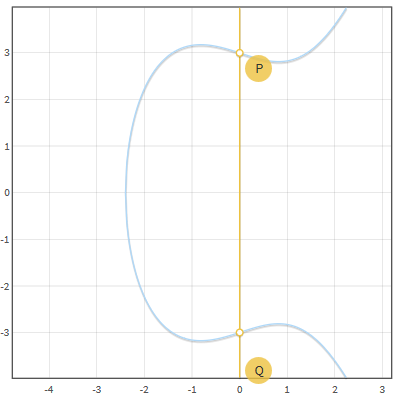
\includegraphics[scale=0.4]{add_opp.png} 
\end{center}

Το σημείο $\mathcal O$. υπάρχει σε \textbf{κάθε κατακόρυφη}
\framebreak

\begin{columns}
\column{0.5\textwidth}
Αν $P \neq Q$ τότε:
\begin{itemize}
\item Θεωρούμε την $\overline{PQ}$
\item Βρίσκουμε το σημείο τομής $R$ με την $\mathcal{E}$.
\item Βρίσκουμε το αντίθετο
\end{itemize}
\column{0.5\textwidth}
\begin{center}
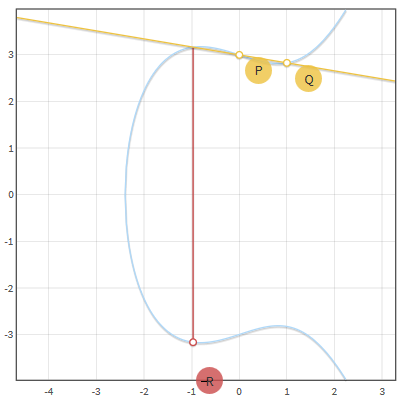
\includegraphics[scale=0.5]{add.png} 
\end{center}
\end{columns}

\framebreak
\begin{columns}
\column{0.5\textwidth}
Αν $P = Q$ τότε:
\begin{itemize}
\item Θεωρούμε την εφαπτομένη στο $P$
\item Βρίσκουμε το σημείο τομής $R$ με την $\mathcal{E}$.
\item Βρίσκουμε το αντίθετο
\end{itemize}
\column{0.5\textwidth}
\begin{center}
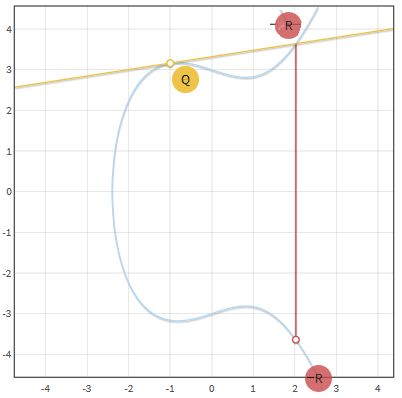
\includegraphics[scale=0.5]{add_same.png} 
\end{center}
\end{columns}
Αλγεβρική αναπαράσταση: Τριτοβάθμιες εξισώσεις με συντεταγμένες
\end{frame}


\begin{frame}{Ομάδα Σημείων Ελλειπτικής καμπύλης}
Τα σημεία μιας ελλειπτικής καμπύλης αποτελούν αβελιανή ομάδα ως προς την πρόσθεση
\begin{itemize}
\item ουδέτερο στοιχείο $\mathcal{O}$
\item αντίθετο στοιχείο $-P$
\item πρόσθεση προσεταιριστική και αντιμεταθετική
\end{itemize}
\end{frame}

\begin{frame}{Πολλαπλασιασμός σημείου με ακέραιο $nP = P + P + \cdots + P$}

\begin{center}
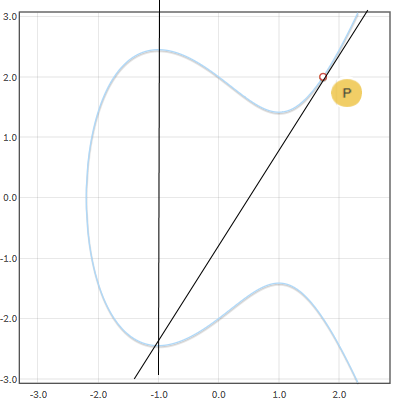
\includegraphics[scale=0.33]{p.png} 
\pause
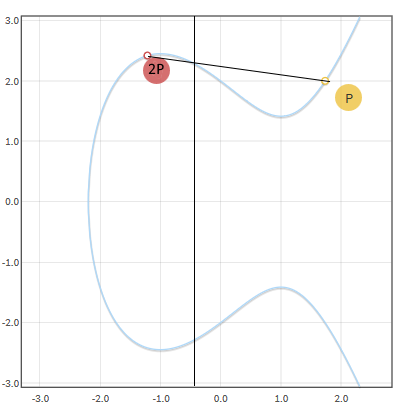
\includegraphics[scale=0.33]{2p.png} \\
\pause
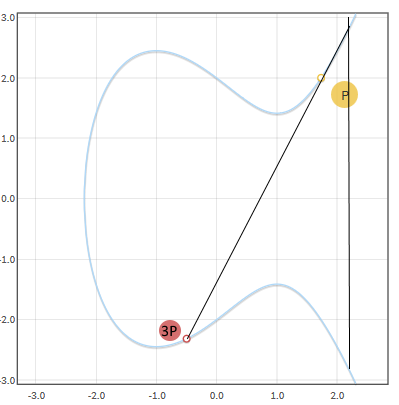
\includegraphics[scale=0.33]{3p.png} 
\pause
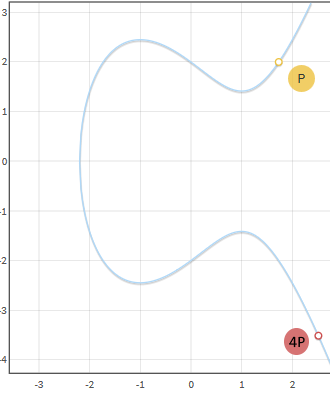
\includegraphics[scale=0.33]{4p.png} 
\end{center}
\end{frame}

\begin{frame}{Double and add}
\magenta{Υπολογισμός $nP$} \\
Απαιτούνται $n-1$ προσθέσεις \\ 

\green{Λύση:} Square and multiply - Double and add
\begin{align*}
17P = P + 16P \\
2P = P+P \\
4P= 2P+2P \\
8P= 4P+4P \\
16P= 8P+8P \\
\end{align*}
 
\end{frame}

\begin{frame}{Ελλειπτικές καμπύλες πάνω από το $\mathbb{F}_p$}

Ορισμός $\mathcal{E}(\mathbb{F}_p)$
\begin{align*}
 \mathcal E = \mathcal O \cup \{  y^2 = x^3 + ax +b \pmod{p},  \\
 (x,y) \in \mathbb{F}_p^2, (a,b) \in \mathbb{F}_p^2:  4a^3+27b^2 \neq 0 \pmod{p} \} 
\end{align*}
\pause
\begin{center}
Παράδειγμα: $y^2 = x^3+1 \pmod{997}$\\
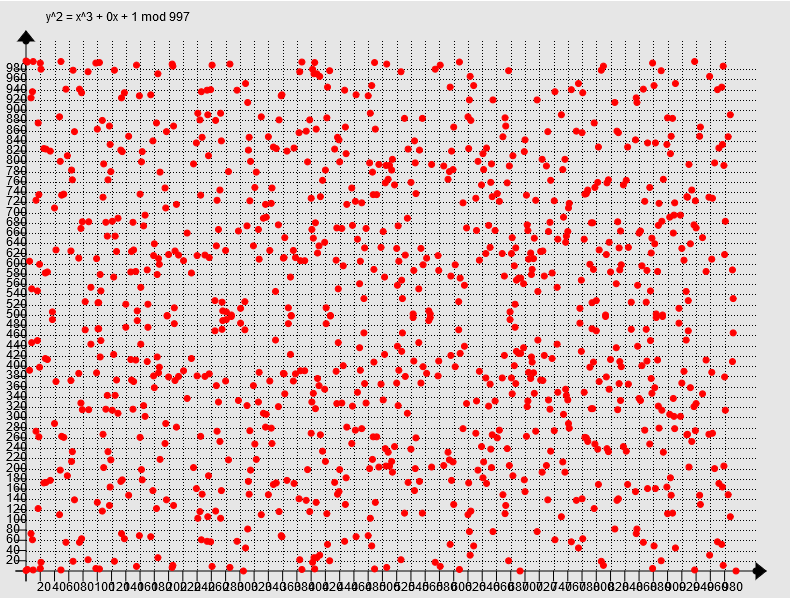
\includegraphics[scale=0.25]{ec997}\\
από \href{http://www.graui.de/elliptic-plot.htm}{Discrete Elliptic Curve Plotter}
\end{center}

\end{frame}

\begin{frame}[allowframebreaks]{Η ομάδα των σημείων $\mathcal{E}(\mathbb{F}_p)$}

Εύρεση τάξης ομάδας

\begin{block}{Εκθετικός αλγόριθμος}
Δοκιμές όλων των $x \in \{0, \cdots, p-1\}$

Έλεγχος ποια ικανοποιούν την εξίσωση της καμπύλης
\end{block}
 
\begin{block}{Θ. Hasse}
$ p+1-2\sqrt{p} \leq\ | \mathcal E(\mathbb{F}_p) | \leq p+1+2\sqrt{p}$
\end{block}

Υπολογισμός: αλγόριθμος Schoof $\in \mathtt{P}$ με βελτιώσεις Elkiens, Atkin (SEA)

\framebreak
\begin{block}{Κυκλικές υποομάδες}
Κάθε σημείο μιας καμπύλης $\mathcal{E}(\mathbb{F}_p)$ παράγει μια κυκλική υποομάδα
\end{block}

\begin{block}{Υπολογισμός τάξης υποομάδας $\mathcal{E}(\mathbb{F}_p)$}
Θεώρημα Lagrange:Η τάξη κάθε υποομάδας διαιρεί την τάξη της ομάδας
\end{block}

Τάξη υποομάδας με σημείο βάσης (γεννήτορα) $P$
\begin{itemize}
\item Εύρεση τάξη ομάδας με αλγόριθμο Schoof
\item Εύρεση των διαιρετών της τάξης, $d$
\item Για σημείο βάσης $P$ εύρεση $min \{d: dP = \mathcal{O}\}$
\end{itemize}

\framebreak

\begin{block}{Εύρεση σημείων βάσης}
Θέλουμε γεννήτορες μεγάλων υποομάδων

\begin{itemize}
\item Ευρεση μεγάλου πρώτου $q \mid |\mathcal{E}|$
\item Υπολογισμός $h=\frac{|\mathcal{E}|}{q}$
\item Επιλογή τυχαίου σημείου $P$
\item Υπολογισμός $G = hP$
\item Αν $G = \mathcal{O}$ επανάληψη
\end{itemize}
\end{block}

\end{frame}

\section{Εφαρμογές στην κρυπτογραφία δημοσίου κλειδιού}

\begin{frame}{Πρόβλημα ECDLP}
\green{\emph{Δίνονται}}: 

\begin{itemize}
\item Μία ελλειπτική καμπύλη $\mathcal E$ ορισμένη πάνω από το $\mathbb{F}_p$ ($p,a,b,\# \mathcal E$)
\item Μία μεγάλη υποομάδα της με τάξη $q$ 
\item ένα σημείο βάσης $G$  και  
\item ένα σημείο  $Y$. 
\end{itemize}
\alert{\emph{Ζητείται}}:
Να βρεθεί, αν υπάρχει, ακέραιος $x$ τέτοιος ώστε $xG=Y$.

\pause
\begin{block}{Εικασία}
Το πρόβλημα ECDLP είναι υπολογιστικά απρόσιτο (όχι σε κάθε καμπύλη)
\end{block}

\end{frame}

\begin{frame}[allowframebreaks]{Ανταλλαγή Κλειδιού ECDH}
\begin{block}{Στόχοι}
\begin{itemize}
\item Κατασκευή κοινού κλειδιού πάνω από δημόσιο κανάλι επικοινωνίας
\item Σε EC: Το κοινό κλειδί είναι σημείο της καμπύλης
\item Δημόσια επικοινωνία και συμφωνία σε σημείο $P$  μιας ελλειπτικής καμπύλης $\mathcal E$
\end{itemize}
\end{block}

Δημόσια Διαθέσιμες Παράμετροι: $(p,a,b,\# \mathcal E,q,G)$
\framebreak
\begin{block}{Πρωτόκολλο}
\begin{itemize}
\item H {Alice} επιλέγει έναν ακέραιο $a \in \{1, \cdots, q-1 \}$
\item Υπολογίζει το $aG \in \mathcal E$ και το δημοσιοποιεί.
\item Ο {Bob} επιλέγει έναν ακέραιο $b \in \{1, \cdots, q-1 \}$ και δημοσιοποιεί το $bG \in \mathcal E$
\item Το δημόσιο κλειδί που θα χρησιμοποιούν στη συνέχεια είναι το $P=a(bG)=b(aG) \in \mathcal E$
\end{itemize}
\end{block}

\end{frame}

\begin{frame}{Κρυπτογραφία Δημοσίου Κλειδιού}
\magenta{Παραλλαγή Κρυπτοσυστήματος ElGamal}

\textbf{Δημιουργία κλειδιών }
\begin{itemize}
\item Δημόσια Διαθέσιμες Παράμετροι: $(p,a,b,\# \mathcal E,q,G)$ \pause
\item Ιδιωτικό κλειδί: Ένας τυχαίος ακέραιος $x \in \{1, \cdots, q-1 \}$ \pause
\item Δημόσιο κλειδί: Το σημείο $Y=xG \in \mathcal{E}$ \pause
\end{itemize}

\textbf{Κρυπτογράφηση}
\begin{itemize}
\item Κωδικοποίηση μηνύματος ως σημείο $P_m$ της $\mathcal{E}$ \pause
\item Επιλέγεται ένας τυχαίος ακέραιος $k \in \{1, \cdots, q-1 \}$ \pause
\item Κρυπτογράφημα: $\enc(Y,P_m) = (kG,P_m+kY)$ \pause
\end{itemize}

\textbf{Αποκρυπτογράφηση}
\begin{itemize}
\item Υπολογισμός \[P_m+kY-x(kG)=P_m\] 
\end{itemize}

\end{frame}

\begin{frame}{Κωδικοποίηση μηνύματος σε σημείο}
\begin{itemize}
\item Hashed Elgamal
\begin{itemize}
\item 1ος τρόπος
\begin{itemize}
\item Χρήση συνάρτησης $\mathcal{H}: \mathcal{E} \Rightarrow \mathcal{M}$
\item Κρυπτογράφηση: $\enc(Y,P_m) = (kG, m\oplus \mathcal{H}(kY))$
\end{itemize}
\item 2oς τρόπος
\begin{itemize}
\item Επιλογή τυχαίου $\alpha$ και αντικατάσταση των bits χαμηλής τάξης του με το $m$
\item Επιλογή ενός από τα δύο πιθανά σημεία της καμπύλης
\end{itemize}
\end{itemize}
\end{itemize}
\end{frame}

\section{Πρακτικά Θέματα}

\begin{frame}{Πρότυπες καμπύλες}
\begin{small}
\begin{block}{Πρότυπο \href{http://csrc.nist.gov/publications/fips/fips186-3/fips_186-3.pdf}{NIST FIPS186-3}}

15 ελλειπτικές καμπύλες. Για παράδειγμα:

\begin{itemize}  
\item \textbf{NIST P-256}
$y^2 = x^3-3x+$\numprint{41058363725152142129326129780047268409114441015993725554835256314039467401291} $\bmod ( 2^{256} - 2^{224} + 2^{192} + 2^{96} - 1) $\\
\pause
Χρήση στην γεννήτρια τυχαιότητας Dual\_EC\_DRBG.
\pause
\item \textbf{NIST P-384 }
$y^2 = x^3-3x+$\numprint{27580193559959705877849011840389048093056905856361568521428707301988689241309860865136260764883745107765439761230575} $\bmod
  (2^{384}- 2^{128} - 2^{96} + 2^{32} - 1) $
\end{itemize}

\alert{Φόβοι για υπονόμευση}
\end{block}
\pause
Εναλλακτικά:\\
\textbf{Secp256k1}  (OpenSSL, Bitcoin) $y^2 = x^3+0x+7 \bmod (2^{256} - 2^{32} - 977)$ \\
\textbf{Curve25519} (OpenSSH) $y^2 = x^3+486662 \cdot x^2+x \bmod (2^{255}-19) $
\end{small}
\end{frame}



\begin{frame}{Επιλογή Καμπύλης}
\alert{To ECDLP δεν είναι δύσκολο σε όλες τις καμπύλες}\\
\pause
Δίνεται μια καμπύλη $(p,a,b,\# \mathcal{E},q,G)$\\
\alert{Πρόβλημα:} Είναι ασφαλής (;)
\pause
\begin{block}{Επαληθευσιμότητα}
\begin{itemize}
\item Επιλογή τυχαίου αριθμού $s$
\item Υπολογισμός $h=\mathcal{H}(s)$
\item Παραγωγή των $a,b$ από το $h$
\item Επαληθευσιμο, αλλιώς $a,b$ από αντιστροφή της σύνοψης
\end{itemize}
\end{block}
\pause
\alert{Αλλά:} Πρέπει το $s$ να είναι πραγματικά τυχαίο!
\begin{block}{Nothing up my sleeve}
Το $s$ προέρχεται από ψηφία του $\pi$, $e$,τριγωνομετρικών αριθμών
\end{block}
\end{frame}




\section{Πηγές}
\begin{frame}[allowframebreaks]{Βιβλιογραφία}
\begin{tiny}
\begin{itemize}
\item St. Zachos and Aris Pagourtzis. Στοιχεία Θεωρίας Αριθμών και Εφαρμογές στην Κρυπτογραφία. Πανεπιστημιακές Σημειώσεις
\item Jonathan Katz and Yehuda Lindell. Introduction to Modern Cryptography (Chapman and Hall/Crc Cryptography and Network Security Series). Chapman
and Hall/CRC, 2007
\item \href{http://goo.gl/b75I29}{Nigel Smart. Introduction to cryptography} 
\item Paar, Christof, and Jan Pelzl. Understanding cryptography: a textbook for students and practitioners. Springer Science-Business Media, 2009.
\item Kiayias, Aggelos  \href{http://crypto.di.uoa.gr/class/Kryptographia/Semeioseis_files/Cryptograph_Primitives_and_Protocols.pdf}{Cryptography primitives and protocols}, UoA, 2015
\item Dan Boneh, Introduction to cryptography, online course
\medskip
\item Neal Koblitz and Alfred J. Menezes, \href{http://eprint.iacr.org/2015/1018.pdf}{A riddle wrapped in an enigma} 
\item Jeremy Kun \href{http://jeremykun.com/2014/02/08/introducing-elliptic-curves/}{Introducing Elliptic Curves}
\item Andrea Corbellini \href{http://andrea.corbellini.name/2015/05/17/elliptic-curve-cryptography-a-gentle-introduction/}{Elliptic Curve Cryptography: a gentle introduction}
\item Torben Pryds Pedersen. Non-interactive and information-theoretic secure verifiable secret sharing. In CRYPTO ’91, pages 129–140, 1991
\item Victor Shoup \href{http://www.shoup.net/papers/expo.pdf}{Why chosen ciphertext security matters}, 1998
\item DR Stinson  
\href{http://anh.cs.luc.edu/331/notes/PohligHellmanp_k2p.pdf}{The Pohlig - Hellman Algorithm}
\end{itemize}
\end{tiny}
\end{frame}

 
\end{document}

